\documentclass{math}

\usepackage{float}
\usepackage{graphicx}
\usepackage{subcaption}

\geometry{letterpaper, margin=0.5in}

\title{Intro to Computer Vision: HW 2}
\author{Alvin Lin}
\date{August 2018 - December 2018}

\begin{document}

\maketitle
\captionsetup{justification=centering}

\subsection*{Part (i)}
My implemented solution fetches the Leung Malik filters from the provided file
and builds the bank of filters as a \( 48\times49\times49 \) matrix before apply
each filter to the grayscaled image. This generates a \( 48\times image_x\times
image_y \) matrix which we transpose to \( image_x\times image_y\times 48 \) so
that we have a 48 dimensional vector for each pixel of the image. In order to
apply the K-means clustering algorithm on it, I flatten this into a \( (image_x
\times image_y) \times 48 \) matrix in two dimensions. Running the K-means
clustering algorithm yields a resulting matrix of the same size containing
the index of the cluster each pixel belongs to. This cluster result matrix is
then reshaped back into the dimensionality of the image to be \( image_x\times
image_y \). From this, we can select the cluster IDs which represent the
animal that we want to segment out and transpose only those segment IDs onto
the background. \par
I ran into many problems implementing this. The provided filter banks gave them
as a \( 49\times49\times48 \) dimensional matrix, and this needed to be
transposed. I ran into several issues because I was using \texttt{numpy}'s
\texttt{reshape()} function on the matrices instead of \texttt{transpose()}.
Additionally, my version of OpenCV had some bugs with \texttt{resize()}, so I
did not resize the source image before transferring it to the background. \par
Some of the edges around the cheetah had gaps and holes due to the texture of
the grass underneath the cheetah. The spots on the cheetah created a lot of
complexity and I had to choose \( k = 40 \) to correctly separate them out.
Using a lower \( k \) value in the K-means clustering algorithm resulted in the
cheetah's back being included in the same cluster as the grassy background. I
achieved a much better result segmenting the gecko. This was probably due to the
higher contrast between the gecko and the white background and the lack of
complex textures like grass.

\subsection*{Part (ii)}
I used scikit-learn's implementation of the K-means clustering algorithm to do
the image segmentation described in part (i), but I also implemented my own
version of the algorithm. My own version was many orders of magnitude slower.
Since I have implemented this algorithm in the past, it was heavily based on my
past work, which can be found here: \\
\url{https://gist.github.com/omgimanerd/ff0b9a8dd225f2d2e94aa4be76bc91d9}

\subsection*{Part (iii)}
\begin{figure}[H]
  \begin{subfigure}{0.33\linewidth}
    \centering
    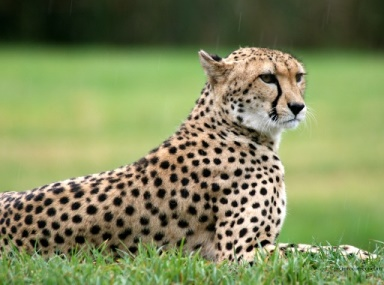
\includegraphics[width=6cm]{assets/hw_02_cheetah.jpg}
    \caption{Original image of cheetah}
  \end{subfigure}
  \begin{subfigure}{0.33\linewidth}
    \centering
    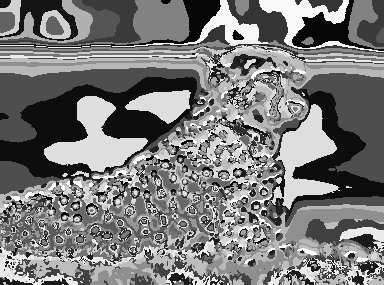
\includegraphics[width=6cm]{assets/hw_02_cheetah_segmentation.png}
    \caption{Segmentation of cheetah image}
  \end{subfigure}
  \begin{subfigure}{0.33\linewidth}
    \centering
    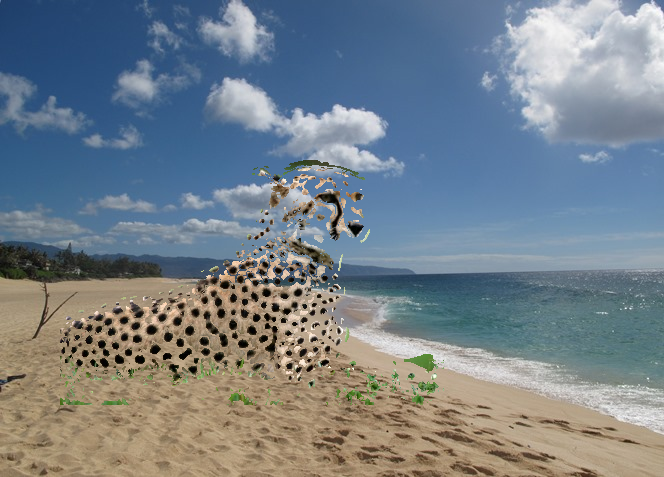
\includegraphics[width=6cm]{assets/hw_02_cheetah_transposed.png}
    \caption{Cheetah transferred to background}
  \end{subfigure}
\end{figure}
\begin{figure}[H]
  \begin{subfigure}{0.33\linewidth}
    \centering
    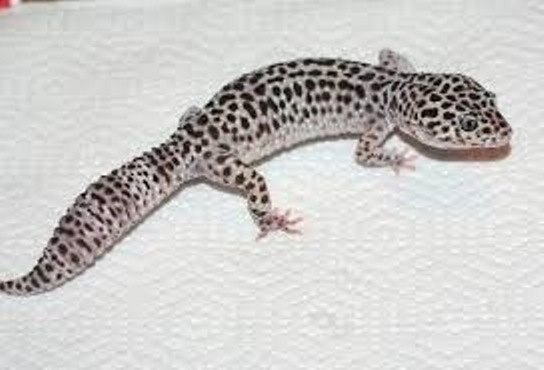
\includegraphics[width=6cm]{assets/hw_02_gecko.jpg}
    \caption{Original image of gecko}
  \end{subfigure}
  \begin{subfigure}{0.33\linewidth}
    \centering
    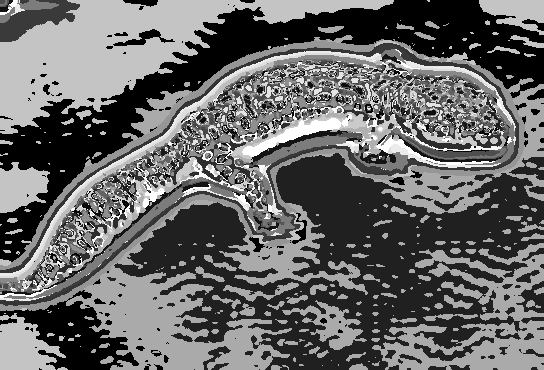
\includegraphics[width=6cm]{assets/hw_02_gecko_segmentation.png}
    \caption{Segmentation of gecko image}
  \end{subfigure}
  \begin{subfigure}{0.33\linewidth}
    \centering
    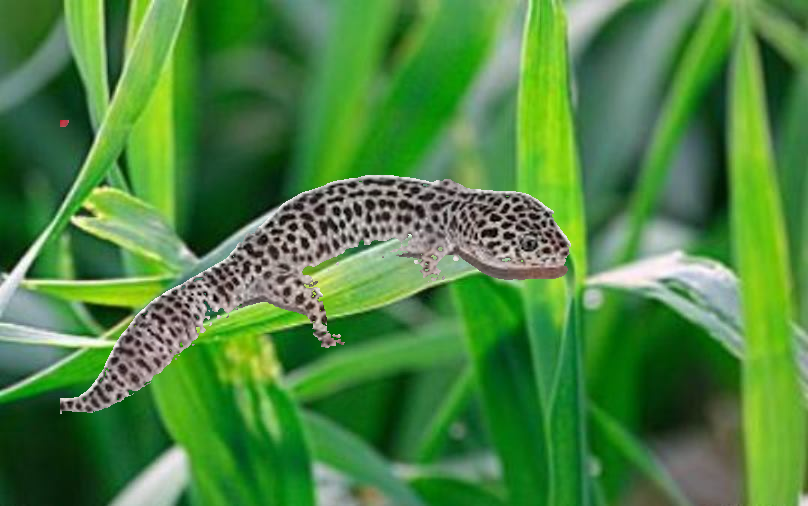
\includegraphics[width=6cm]{assets/hw_02_gecko_transposed.png}
    \caption{Gecko transferred to background}
  \end{subfigure}
\end{figure}

\subsection*{Part (iv)}
The segmentation of the cheetah has many holes in it most likely due to the
coloration of the cheetah. The white regions around the anterior edge and the
mouth of the cheetah blend with the background and do not form a clear edge
to be detected by the filter bank. This is evident in the visualization of the
cheetah's segmentation. Note that the light regions around the cheetah's head
also blend with the horizon lines in the background. \par
It seems like oversegmenting the image resulted in more distinctly separated
regions, so choosing a higher \( k \) for the K-means clustering algorithm
would likely result in less ambiguity between the animal and the background
region. Increasing the contrast of the image would probably help with the
segmentation.

\begin{center}
  If you have any questions, comments, or concerns, please contact me at
  alvin@omgimanerd.tech
\end{center}

\end{document}
